%% hugo-title: LaTeX Blog Example
%% hugo-date: 2026-07-14
%% hugo-draft: false

\documentclass[11pt]{article}
%% Shared Tufte-inspired preamble — matches site colorway
\usepackage[T1]{fontenc}
\usepackage{lmodern}
\usepackage{amsmath,amssymb}
\usepackage{graphicx}
\usepackage{booktabs}
\usepackage{microtype}
\usepackage[
  paperwidth=6.5in,
  top=1.4in,
  bottom=1.4in,
  left=1in,
  right=2.75in,
  marginparwidth=1.75in,
  marginparsep=0.2in
]{geometry}

\usepackage{xcolor}
\definecolor{textcolor}{RGB}{39,39,39}
\definecolor{linkcolor}{RGB}{26,13,171}
\definecolor{rulecolor}{RGB}{39,39,39}

\usepackage[colorlinks=true,linkcolor=linkcolor,citecolor=linkcolor,urlcolor=linkcolor]{hyperref}

\usepackage{tikz}
\usetikzlibrary{arrows.meta,calc}

\pagestyle{empty}
\setlength{\parindent}{0pt}
\setlength{\parskip}{0.65\baselineskip}
\color{textcolor}

%% Section spacing (Tufte-inspired, no extra packages)
\makeatletter
\renewcommand\section{\@startsection{section}{1}{0pt}{1.25\baselineskip}{0.5\baselineskip}{\large\bfseries\color{textcolor}}}
\renewcommand\subsection{\@startsection{subsection}{2}{0pt}{1\baselineskip}{0.35\baselineskip}{\normalsize\bfseries\color{textcolor}}}
\makeatother

%% Margin notes (Tufte sidenotes)
\newcommand{\sidenote}[1]{\marginpar{\footnotesize\color{textcolor}#1}}

%% TL;DR block
\newcommand{\tldr}[1]{%
  \noindent{\color{linkcolor}\textit{TL;DR}}\textit{ #1}\par\vspace{0.5\baselineskip}%
}

%% Figure styling
\usepackage{caption}
\captionsetup{
  font=small,
  labelfont=bf,
  textfont=it,
  skip=0.5\baselineskip
}


\begin{document}

\tldr{Blog posts can be authored in \LaTeX{} and compiled to HTML with Tufte-style layout and site colors.}

\section{Writing in \LaTeX}

This post is compiled from \texttt{tex/blog/latex-example.tex}. Body text uses Computer Modern at the same gray tone as the rest of the site, and links use the site blue \textcolor{linkcolor}{rgb(26, 13, 171)}.

\section{Math}

Display equations render via MathJax:
\begin{equation}
  y_i = \alpha + \beta x_i + \varepsilon_i, \qquad \varepsilon_i \sim \mathcal{N}(0, \sigma^2).
\end{equation}

\section{A TikZ figure}

\begin{figure}[ht]
\centering
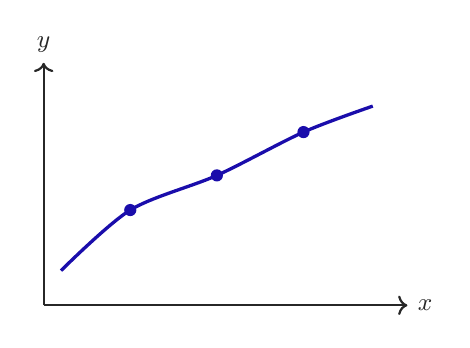
\begin{tikzpicture}[scale=1.1, every node/.style={color=textcolor, font=\small}]
  \draw[->, thick, color=rulecolor] (0,0) -- (4.2,0) node[right] {$x$};
  \draw[->, thick, color=rulecolor] (0,0) -- (0,2.8) node[above] {$y$};
  \draw[linkcolor, very thick, smooth] plot coordinates {(0.2,0.4) (1,1.1) (2,1.5) (3,2.0) (3.8,2.3)};
  \fill[linkcolor] (1,1.1) circle (2pt);
  \fill[linkcolor] (2,1.5) circle (2pt);
  \fill[linkcolor] (3,2.0) circle (2pt);
\end{tikzpicture}
\caption{A simple TikZ line plot in site colors.}
\end{figure}

\sidenote{Margin notes echo Tufte's sidenotes and sit in the wide right margin.}

\section{Tables}

\begin{table}[ht]
\centering
\begin{tabular}{@{}lrr@{}}
\toprule
Variable & Mean & Std.\ Dev. \\
\midrule
Outcome  & 4.21 & 1.08 \\
Treatment & 0.34 & 0.47 \\
\bottomrule
\end{tabular}
\caption{Summary statistics.}
\end{table}

\end{document}
